% タイトル
\chapter{方程式の解}
\vspace{-45pt} %高さ調整
\begin{flushright}
  {\bf \large 理工学部 電子工学科 1回生} \\ \vspace{3pt} %所属
  {\bf \large 辻 新也} \\ \vspace{30pt} %名前
\end{flushright}

% 序論
\section*{はじめに}
数学の入試問題の中には単に「入試問題」として解いているだけでは気づかない背景があり、それを調べてみるとまるでマジックの種明かしを見ているようなおもしろさがあります。\par
次の問は僕が受験生の時に出会った問題です。まずは自力で考えてみましょう。

%
\section*{問1}
\addcontentsline{toc}{section}{問1}

\begin{screen}
三次の整式$f(x) = x^3 + x^2 +px +q(ただしp \neq q,q \neq 0)$、および$g(x) = \frac{-1}{x+1}$が次の条件($\ast$)を満たすとする。
\begin{center}
  ($\ast$)\quad $f(x) = 0$の任意の解$\alpha$に対して$g(x)$も$f(x) = 0$の解である。
\end{center}
\begin{enumerate}
  \item $p,q$の値を求めよ。
  \item $f(x) = 0$は$-2<x<2$の範囲に三つの実数解をもつことを示せ。
  \item $f(x) = 0$の任意の解を$2 \cos \theta$とするとき、$2\cos 2\theta 、2 \cos 3\theta$も解であることを示せ。
  \item $2\cos \theta (0<\theta<\pi)$が$f(x) = 0$の解であるとき、$\theta$の値を求めよ。
\end{enumerate}
\end{screen}
%
\subsection*{解答}
\noindent [1]\quad $x = 0,-1$は$f(x)=0$を満たさないので、$x = 0,-1$は$f(x)=0$の解ではない。
よって$\alpha \neq 0,-1$\\
($x = 0$が解と仮定すると、$f(0) = q = 0$となり、$q \neq 0$に矛盾、$x = -1$が解と仮定すると、$f(-1) = -p + q = 0$すなわち$p=q$となり、$p \neq q$に矛盾。)\\
ここで、条件($\ast$)より$g(g(\alpha))$も$f(x) = 0$の解である。\\
(条件($\ast$)より、任意の解を$g(\alpha)$とすると、$g(g(\alpha))$も解となることが分かる。$g(g(g(\alpha)))$も同様。)\\
よって、$g(\alpha) = \frac{-1}{\alpha + 1}$が解であるから
\begin{align*}
 g(g(\alpha)) = \frac{-1}{\frac{-1}{\alpha + 1}+1} = - 1 - \frac{1}{\alpha}\\
 g(g(g(\alpha))) = \frac{-1}{-1-\frac{-1}{\alpha}+1} = \alpha
\end{align*}
も共に解である。\\
($g(g(g(\alpha)))$が$\alpha$となり$\alpha \rightarrow g(\alpha) \rightarrow g(g(\alpha)) \rightarrow g(g(g(\alpha))) = \alpha$と循環します。)\\
$f(x) = 0$の解が$\alpha,\frac{-1}{\alpha + 1},-1-\frac{1}{\alpha}$となるから、解と係数の関係より
\begin{align*}
  \begin{cases}
  \, p = \dfrac{-\alpha}{\alpha + 1}-\dfrac{1}{\alpha}+\alpha +1\\
  \, q = -1\\
  \, \alpha^3 + \alpha^2 -2\alpha -1 = 0
  \end{cases}
\end{align*}
よって、$p = -2,\,q=-1$。
\begin{flushright}
  $\square$
\end{flushright}

\noindent [2]\quad {[1]}より$f(x) = x^3 + x^2 -2x -1$。$f(x)$は連続関数で
\begin{align*}
  f(-2) &= -1 < 0,\\
  f(-1) &= 1 > 0,\\
  f(0) &= -1 < 0,\\
  f(2) &= 7 > 0
\end{align*}
となり、$f(x) = 0$は$-2<x<2$の範囲に三つの実数解をもつ。\\
(それぞれ$-2<x<-1,-1<x<0,0<x<2$に一つずつ)
\begin{figure}[H]
  \centering
  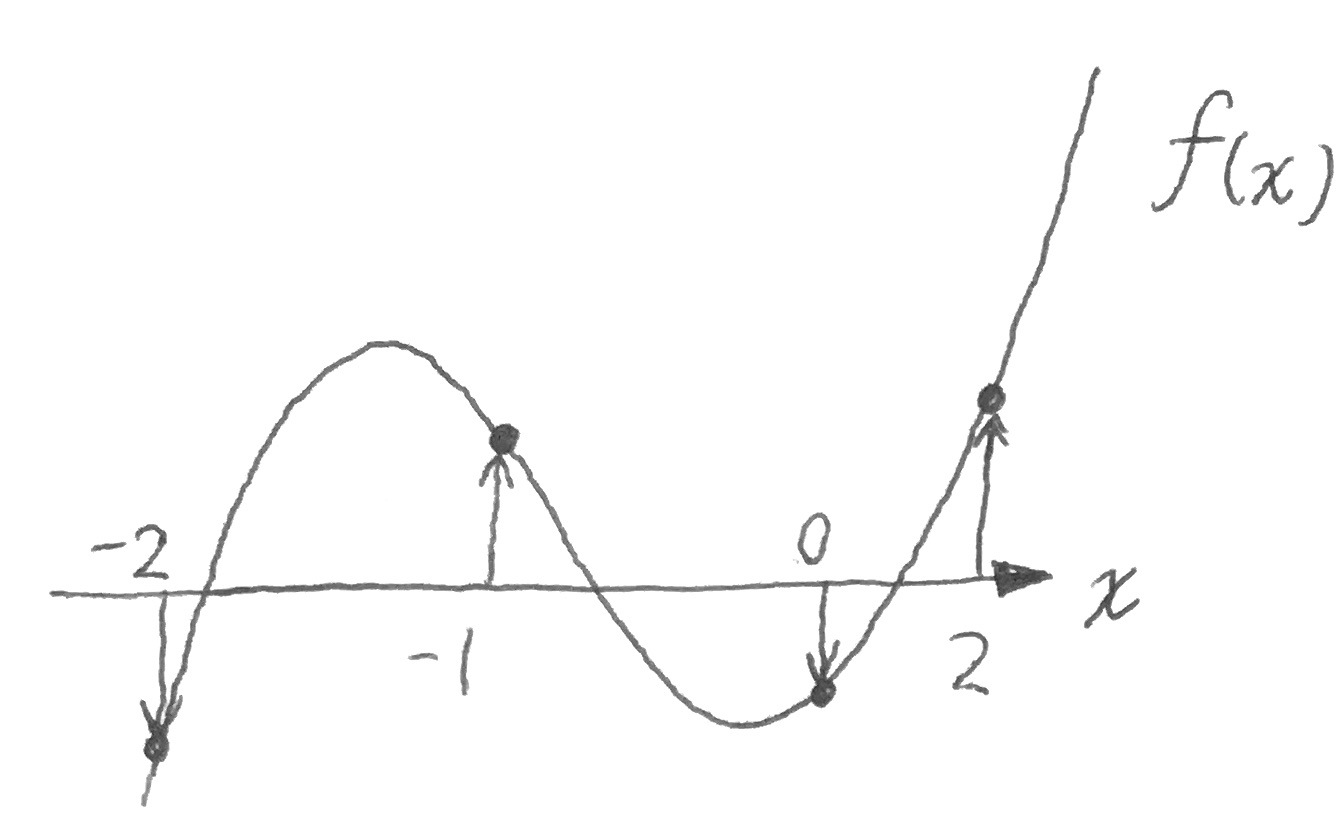
\includegraphics[width=5cm]{tuzi/image/0}
\end{figure}
\begin{flushright}
  $\square$
\end{flushright}

\noindent [3] 任意の解を$2\cos \theta$とすると、$\alpha = 2\cos \theta$とおける。$f(\alpha) = 0$より
\begin{align}
  \label{eq:toi1-1}
\alpha^3 + \alpha^2 -2\alpha -1 = 0
\end{align}
2倍角、3倍角の公式より
\begin{align}
2\cos 2\theta &= 4\cos^2 \theta -2 = \alpha^2 -2 \label{eq:toi1-2}\\
2\cos 3\theta &= \alpha^3 -3\alpha \label{eq:toi1-3}
\end{align}
ここで
\begin{eqnarray*}
  g(\alpha) &=& \frac{-1}{\alpha + 1}\\
  &=&\frac{\alpha^3 + \alpha^2 - 2\alpha -1}{\alpha + 1} \qquad\quad \text{(式(\ref{eq:toi1-1})より)}\\
  &=&\frac{\alpha^2(\alpha + 1) -2(\alpha + 1)}{\alpha + 1}\\
  &=&\alpha^2 -2\\
  &=&2 \cos 2\theta \qquad\qquad\qquad\quad\,\,\,\, \text{(式(\ref{eq:toi1-2})より)}
\end{eqnarray*}
また
\begin{eqnarray*}\hspace{20mm}
g(g(\alpha)) &=& -1 -\frac{1}{\alpha}\\
&=& \frac{(\alpha-1)(\alpha^3 + \alpha^2-2\alpha-1) -\alpha -1}{\alpha} \qquad \text{(式(\ref{eq:toi1-1})より)}\\
&=& \alpha^3 -3\alpha\\
&=& 2\cos 3\theta \hspace{50mm} \text{(式(\ref{eq:toi1-3})より)}
\end{eqnarray*}
よって$g(\alpha) = 2 \cos 2 \theta,\, g(g(\alpha)) = 2\cos 3\theta$となるので、$2\cos 2\theta,\, 2\cos 3\theta$は$f(x) = 0$の解である。
\begin{flushright}
  $\square$
\end{flushright}

\noindent [4] $2\cos \theta$ が$f(x) = 0$の解であるとき、[3]より$2\cos 2\theta$も解で、$2\cos 4\theta$も解である。
\begin{eqnarray*}
2\cos 2\theta &=& g(2 \cos \theta)\\
2\cos 3\theta &=& g(g(2\cos \theta))
\end{eqnarray*}
よって
\begin{eqnarray*}
2\cos 3 \theta = g(2\cos 2\theta)
\end{eqnarray*}
となるから
\begin{eqnarray*}
2\cos 4\theta &=& 2\cos 3\theta\\
\cos 4\theta &=& \cos 3\theta\\
4\theta &=& \pm 3 \theta + 2n\pi\ \ \ \text{($n$は整数)} \\
\end{eqnarray*}
$0<\theta<\pi$より
$$ \theta = \frac{2}{7}\pi,\,\frac{4}{7}\pi,\,\frac{6}{7}\pi $$
(つまり$f(x) = 0$の解は、$2\cos \frac{2}{7}\pi,\, 2\cos \frac{4}{7}\pi,\, 2\cos \frac{6}{7}\pi$ということ。)
\begin{flushright}
  $\square$
\end{flushright}

以下の問を用いてさらに考察していきましょう。

%
\section*{問2}
\addcontentsline{toc}{section}{問2}

\begin{screen}
問1の方程式$x^3+x^2-2x-1 =0$について$x =z + \frac{1}{z}$として、$z$の方程式であらわせ。さらに、その$z$の方程式を$h(z) = 0$として$(z-1)\cdot h(z) = 0$を解け。(解は$\cos,\, \sin,\, i$を用いてよい)
\end{screen}
%
\subsection*{解答}
\vspace{-10mm}
\begin{align*}
  & \left(z+\frac{1}{z}\right)^3+\left(z+\frac{1}{z}\right)^2-2\left(z+\frac{1}{z}\right)-1\\
  =& \,\, z^3+\frac{1}{z^3}+3z+\frac{3}{z}+z^2+\frac{1}{z^2} +2-2z -\frac{2}{z} -1\\
  =& \,\, z^3+z^2+z+1+\frac{1}{z} +\frac{1}{z^2}+\frac{1}{z^3} = 0
\end{align*}
両辺に$z^3(\neq 0)$をかけて
\begin{eqnarray*}
  z^6 + z^5 + z^4 + z^3 + z^2 +z + 1 = 0
\end{eqnarray*}
(なんと、$z$の相反方程式(しかも、すべての係数が1)が現れました。)\par
さらに
\begin{align*}\hspace{-30mm}
  (z-1)(z^6+z^5+z^4+z^3+z^2+z+1) &= 0\\
  z^7 -1 &= 0\\
  z^7 &= 1
\end{align*}
(zは1の7乗根ですね!)
$$ z = r(\cos \theta + i\sin \theta) \qquad (r>0,\, 0\leqq \theta < 2\pi) $$
とおくと
\begin{eqnarray*}
z^7 = r^7(\cos 7\theta + i\sin 7\theta)
\end{eqnarray*}
よって$z^7 = 1$は
\begin{eqnarray*}
r^7(\cos 7\theta + i\sin 7\theta) = \cos 0 + i\sin 0
\end{eqnarray*}
よって
$r^7 = 1$より$r=1$。\\
また、$7 \theta = 2n\pi \,\, (n = 0,1,2 \cdot \cdot \cdot ,6)$より$\theta = \frac{2n\pi}{7}$。\\
ゆえに$z_n = \cos\frac{2n\pi}{7} + i\sin\frac{2n\pi}{7}$\,\,($n = 0,1,\cdot \cdot \cdot,6$)と表せるから
\begin{align*}
  \begin{cases}
    \, z_0 = 1 \\
    \, z_1 = \cos\frac{2}{7}\pi + i\sin\frac{2}{7}\pi\\
    \, z_2 = \cos\frac{4}{7}\pi + i\sin\frac{4}{7}\pi\\
    \, z_3 = \cos\frac{6}{7}\pi + i\sin\frac{6}{7}\pi\\
    \, z_4 = \cos\frac{8}{7}\pi + i\sin\frac{8}{7}\pi\\
    \, z_5 = \cos\frac{10}{7}\pi + i\sin\frac{10}{7}\pi\\
    \, z_6 = \cos\frac{12}{7}\pi + i\sin\frac{12}{7}\pi
  \end{cases}
\end{align*}
\begin{flushright}
  $\square$
\end{flushright}

\vspace{10mm}
ここで、
$$x = z + \frac{1}{z} = z + \overline{z}$$
なので$z_1,z_2,z_3$を代入すると、それぞれ$2\cos \frac{2}{7}\pi,\, 2\cos\frac{4}{7}\pi,\, 2\cos\frac{6}{7}\pi$となり$f(x) = 0$の解になりますね。$z_4,z_5,z_6$を代入してもそれぞれ同じ値になりますね。
\begin{figure}[H]
  \centering
  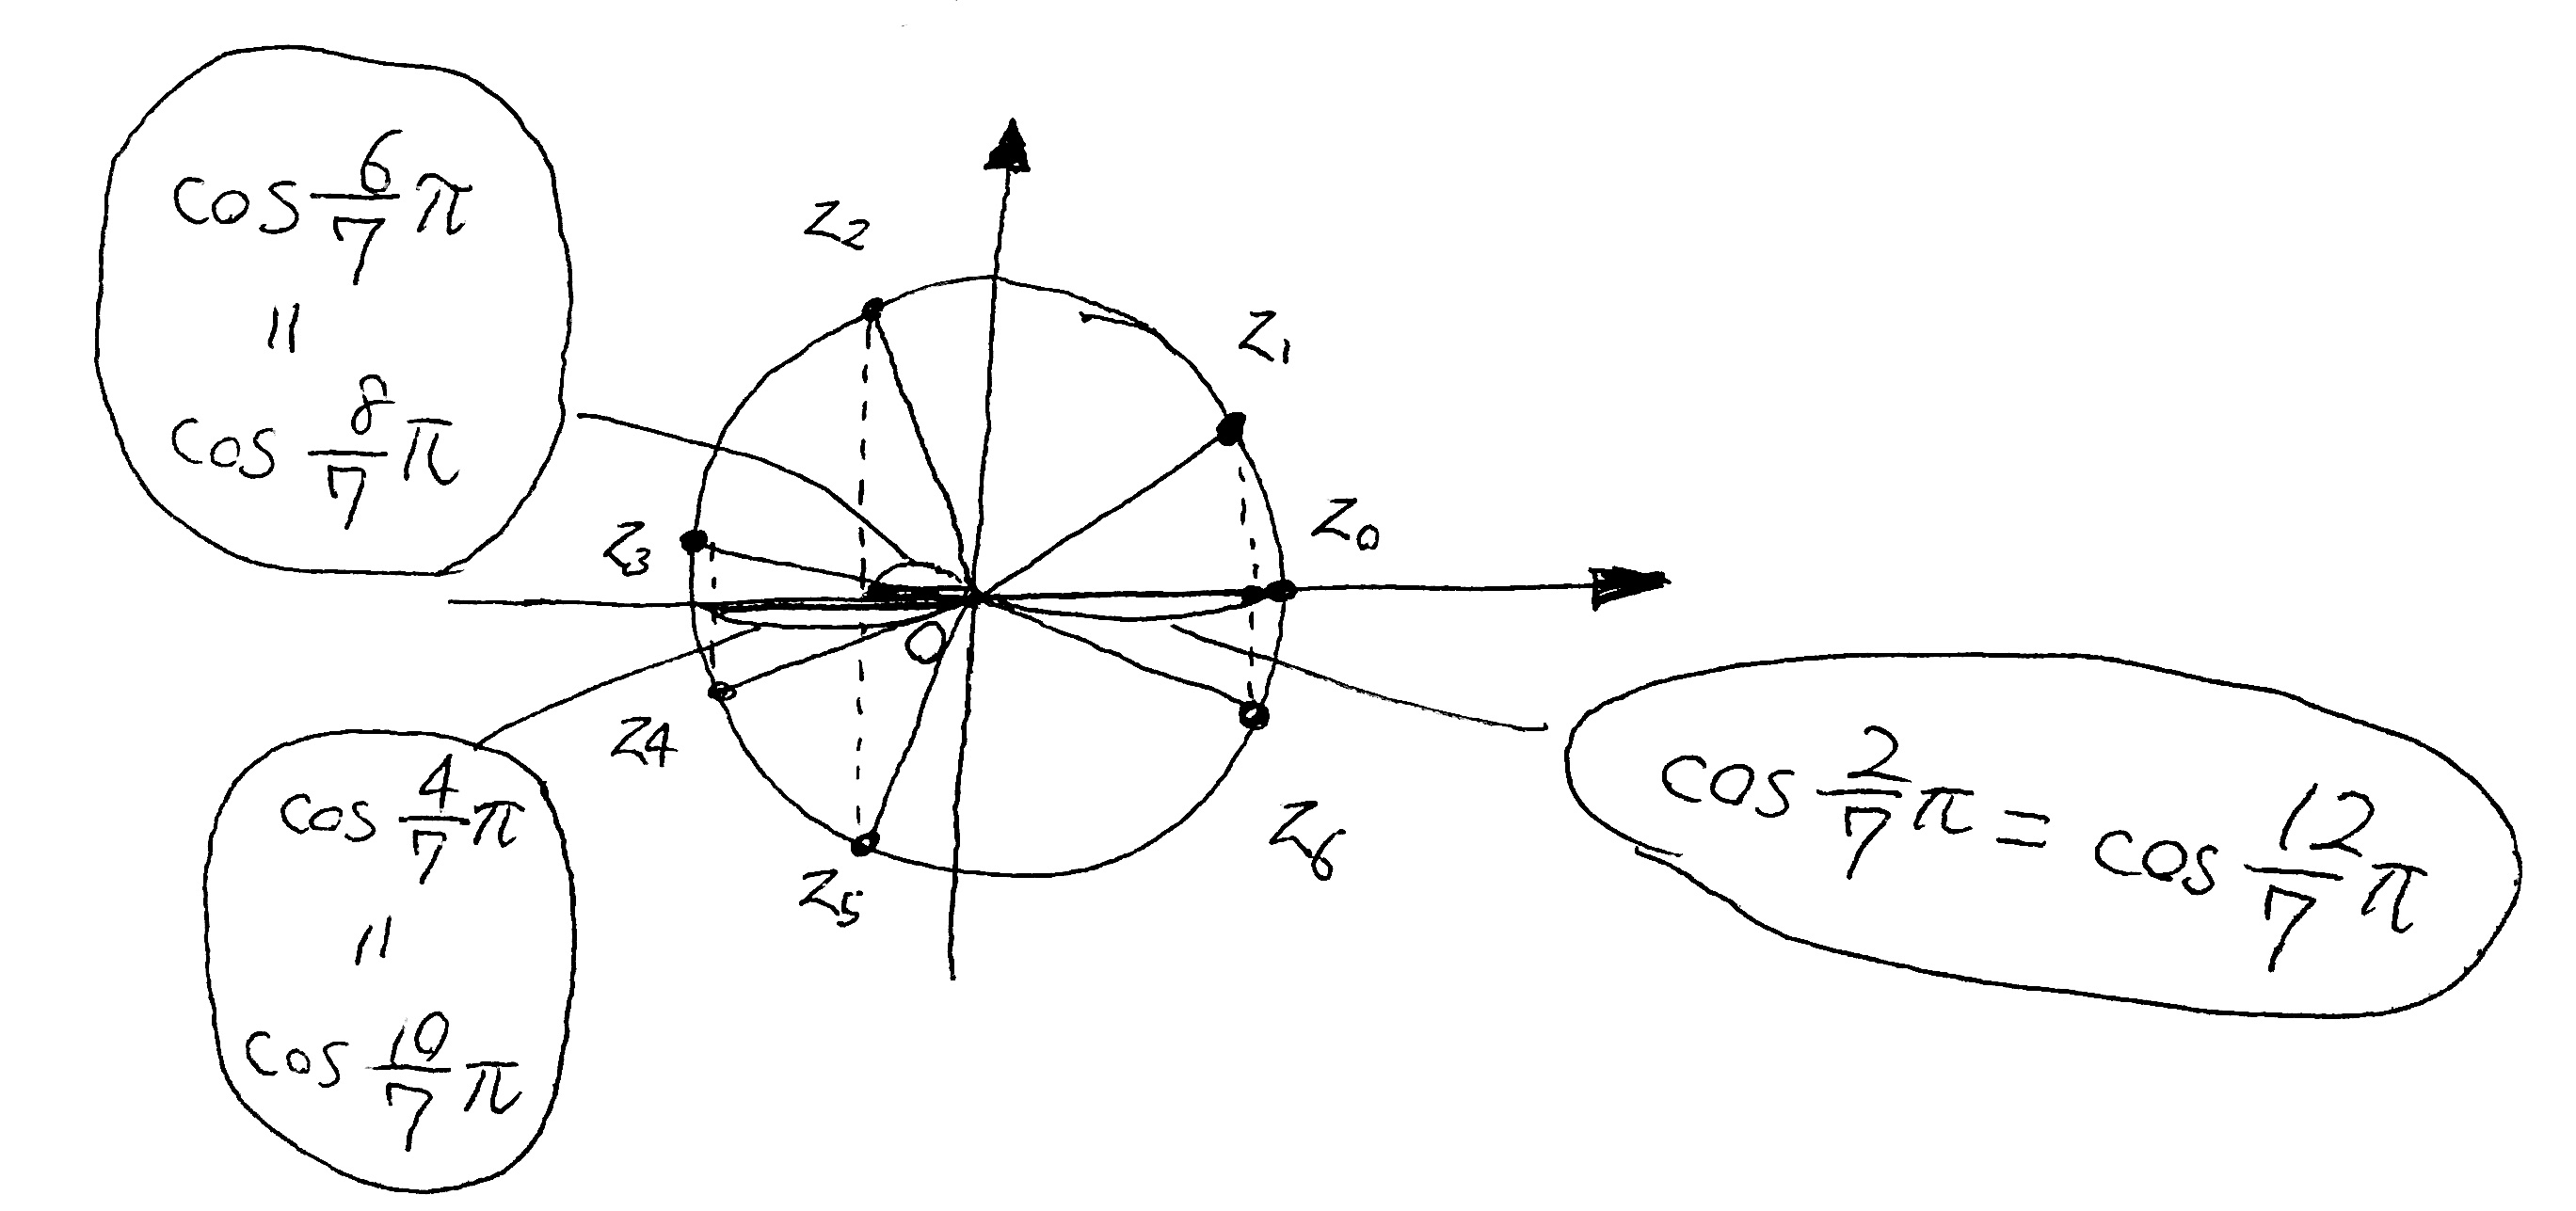
\includegraphics[width=10cm]{tuzi/image/1}
\end{figure}\par
似たような考え方で$\cos \frac{2}{5}\pi$の値を求めることができます。

%
\section*{問3}
\addcontentsline{toc}{section}{問3}
\begin{screen}
方程式$x^5 = 1$を用いて$\cos\frac{2}{5}\pi,\cos\frac{4}{5}\pi$の値を求めよ
\end{screen}
%
\subsection*{解答}
\begin{align*}
  x^5 &= 1\\
  x^5 -1 &= 0\\
  (x-1)(x^4+x^3+x^2+x+1) &= 0 \hspace{10zw}
\end{align*}
$x^4+x^3+x^2+x+1 = 0$について、$x \neq 0$より
$$
x^2 + x +1 + \frac{1}{x} + \frac{1}{x^2} = 0
$$
$t = x + \frac{1}{x}$とおくと
\begin{align*}
  t^2 -2 +t+1 &= 0\\
  t^2 + t - 1 &= 0
\end{align*}
よって
$$t = \frac{-1 \pm \sqrt{5}}{2}$$
また、$z = r(\cos \theta + i\sin \theta)$  ($r>0,\, 0\leqq \theta < 2\pi$)として
\begin{align*}
  r^5(\cos 5 \theta + i\sin 5 \theta) = \cos 0 + i\sin 0, \\
  r= 1,\quad \theta = \frac{2n\pi}{5}\,\,\,(n=0,1,2,3,4), \\
  x_n = \cos\frac{2n\pi}{5}+i\sin\frac{2n\pi}{5} \qquad
\end{align*}
よって
$$ t= x + \frac{1}{x} = 2\cos\frac {2n\pi}{5}$$
以上より
\begin{align*}
  \cos\frac{2}{5}\pi = \frac{\sqrt{5} - 1}{4}, \\
  \cos \frac{4}{5}\pi = -\frac{\sqrt{5} + 1}{4}
\end{align*}
\begin{flushright}
  $\square$
\end{flushright}

\begin{wrapfigure}{r}{40mm}
  \centering
  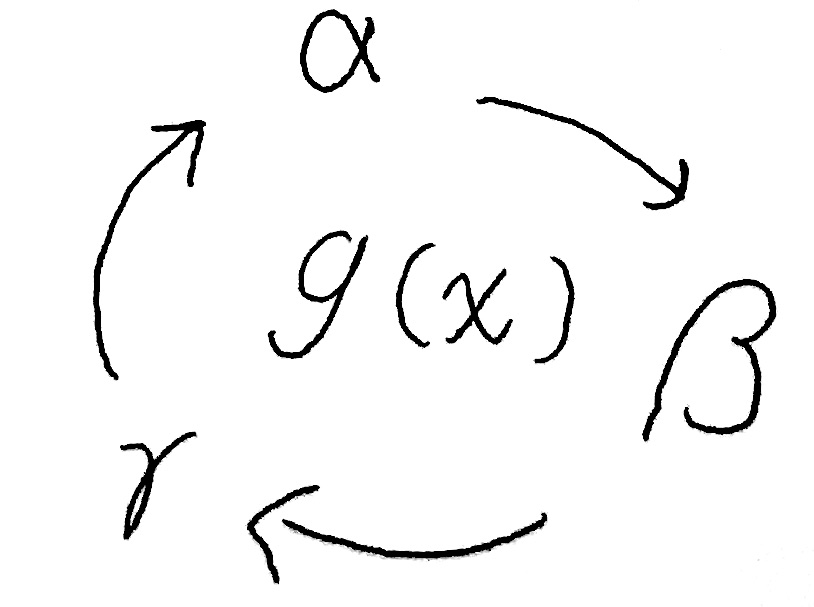
\includegraphics[width=25mm]{tuzi/image/2}
\end{wrapfigure}
問1で$f(x)$の解を$\alpha,\beta,\gamma$とすると、$g(x)$を用いて$\beta = g(\alpha),\gamma = g(\beta),\alpha = g(\gamma)$と循環しました。これについて考えてみましょう。


%
\section*{問4}
\addcontentsline{toc}{section}{問4}

\begin{screen}
  二次方程式$x^2+px+q = 0$の解$\alpha,\beta$(虚数解でもOKだが、重解は除く($\alpha \neq \beta$に矛盾))について$G(x) = ax +b$として、$G(\alpha) = \beta, G(\beta) = \alpha$が成立する$a,b$を求めよ。
\end{screen}
%
\subsection*{解答}
\begin{center}
  \begin{tabular}[t]{rl}
  \ldelim\{{2}{0pt}[]& \parbox[t]{5em}{
  $a\alpha+b=\beta$}\\
  & $a\beta+b=\alpha$
  \end{tabular}
\end{center}
2式から
$$a(\alpha -\beta)= \beta-\alpha$$
$\alpha \neq \beta$より
$$a = -1$$
このとき
\begin{align*}
  -(\alpha+\beta)+2b = \alpha + \beta \\
  b=\alpha+\beta
\end{align*}
よって、解と係数の関係より
$$\qquad b= -p$$
ゆえに
$$G(x) = -x-p$$
\begin{figure}[H]
  \centering
  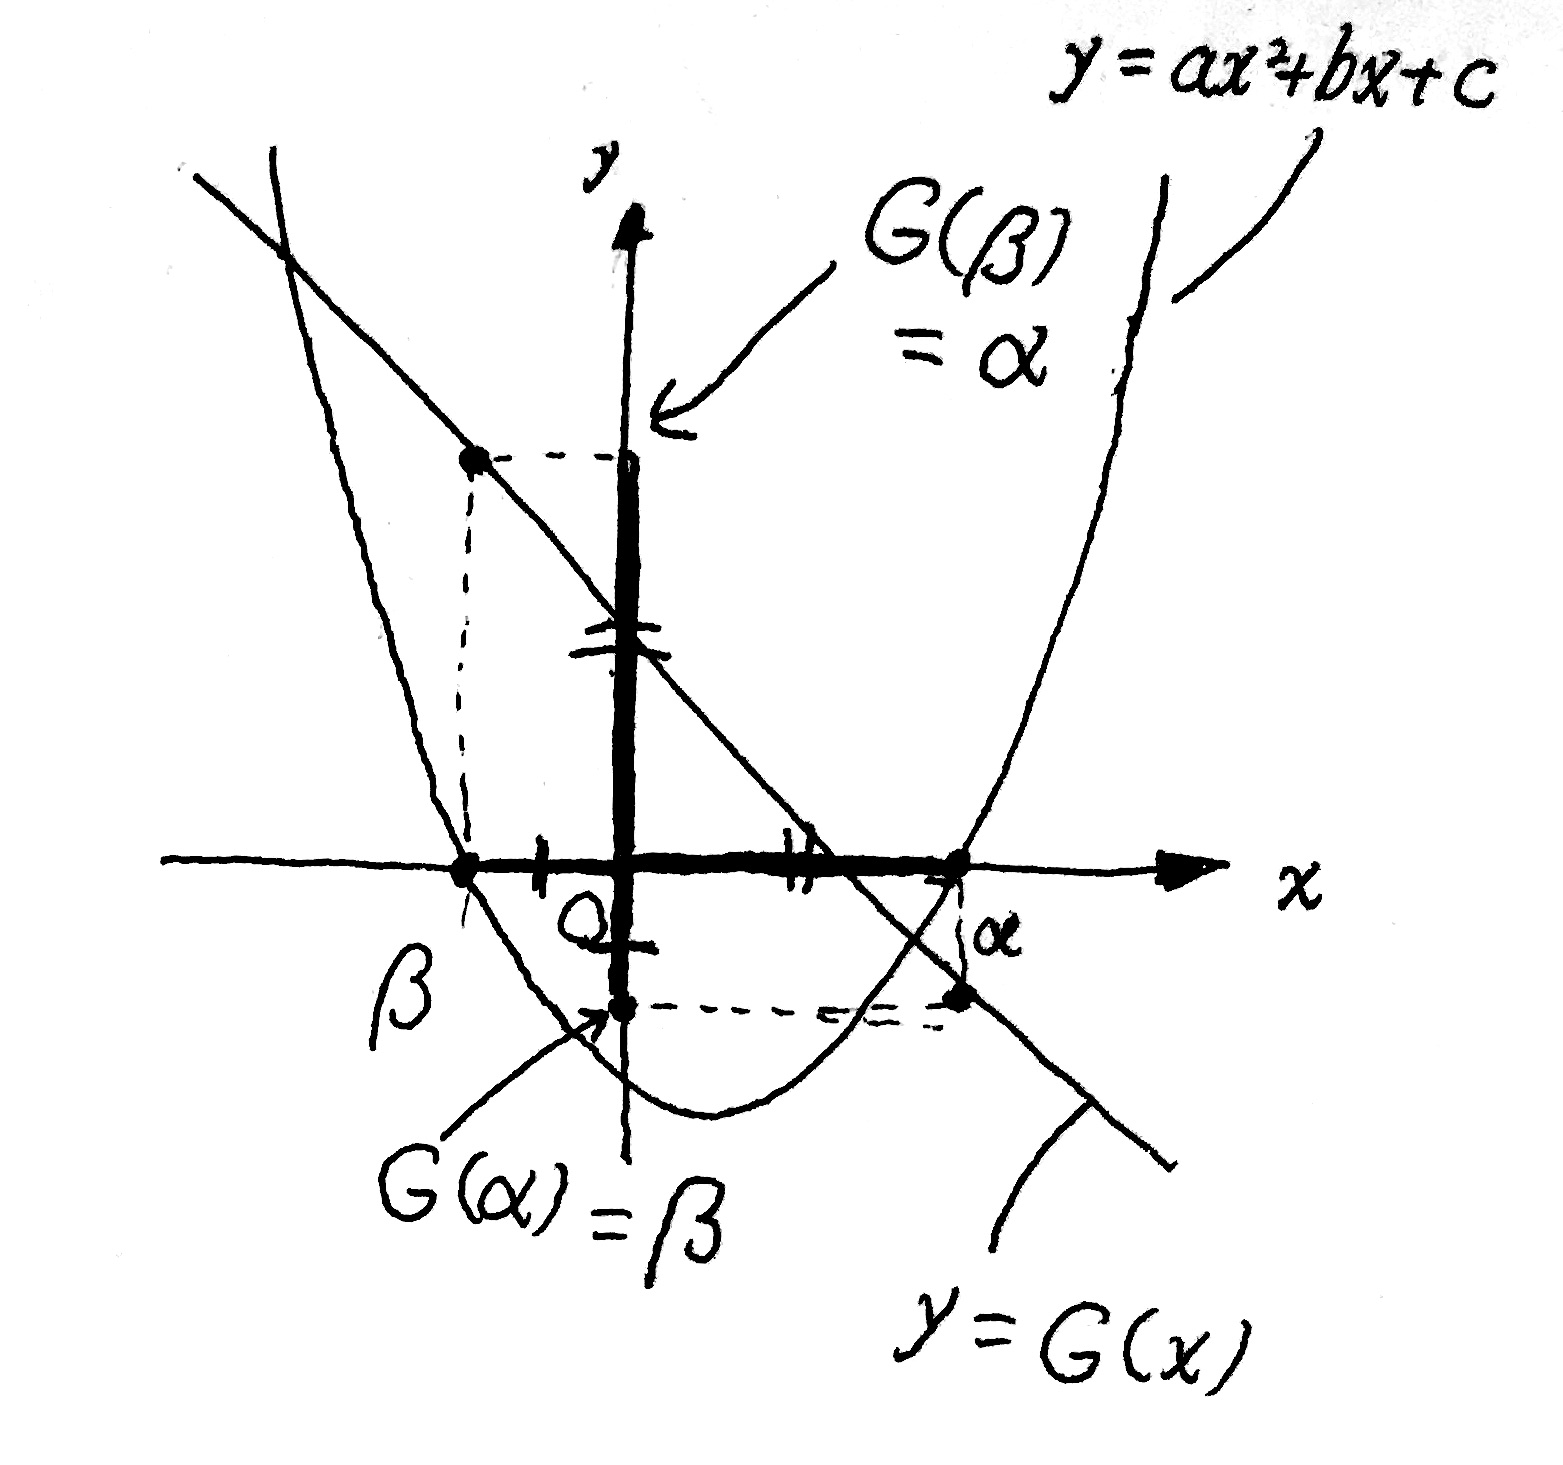
\includegraphics[width=6cm]{tuzi/image/4}
\end{figure}
\begin{flushright}
  $\square$
\end{flushright}

例えば$x^2+2x-8 = 0$について
$$G(x) = -x+2$$
となり解は$x = -2,4$なので
$$ G(-2) = -(-2)+2 = 4,\,\, G(4) = -4 +2 = -2 $$
と循環していますね。($G(G(-2)) = -2$)

\vspace{2zw}
\begin{itembox}[l]{\bf 二次方程式の解の循環}
  二次方程式$x^2+px+q = 0$の解の循環の式は$g(x) = -x -p$
\end{itembox}
\begin{itemize}
  \item 二次方程式の解の循環式では$g(g(x)) = x$が成り立ちます。
  \item 三次方程式の解の循環式はどうでしょう。導出は複雑すぎるので省きますが、解と係数の関係、判別式などを用いて連立すると導出できます。
\end{itemize}
\begin{itembox}[l]{\bf 三次方程式の解の循環}
三次方程式$x^3+px+qx+r = 0$の解の循環の式は$g(x) = ax^2+bx+c$。\\
ただし、
\begin{align*}
  s &= \pm \sqrt{p^2q^2-4p^3r-4q^3+18pqr-27r^2}\\
  & \hspace{40mm} \text{(ルートの中は判別式)}\\
  a &= \frac{3q-p^2}{s}\\
  b &= \frac{1}{2}\left(\frac{7pq-2p^3-qr}{s} - 1\right)\\
  c &= \frac{1}{2}\left(\frac{4q^2-p^2q-3pr}{s} - p\right)
\end{align*}
また
\begin{align*}
  x^3 + px+qx +r = g(x)h(x) +r \quad \text{($h(x)$は商、$r$は余り)}
\end{align*}
より$g(x)h(x) + r = 0$として\\
\[
g(x) = -\frac{r}{h(x)}
\]
より$-\frac{r}{h(x)} \quad \text{(一次分数関数)}$も解の循環式
\end{itembox}

これを用いて問1の$x^3+x^2-2x-1 = 0$の解の循環式は二次関数の形では
\[
g_1(x) = x^2 -2\ \ または\ \ g_2(x) = -x^2-x+1
\]
一次分数関数の形では
\[
g_1(x)よりh_1(x) =\frac{-1}{x+1}
\]
(問1と同じ循環式が出てきましたね)
\[
g_2(x)よりh_2(x)=-\frac{x+1}{x}
\]
$g_1(x),g_2(x),h_1(x),h_2(x)$の違いは何でしょうか。解$\alpha$を代入してみると
\begin{figure}[H]
  \centering
  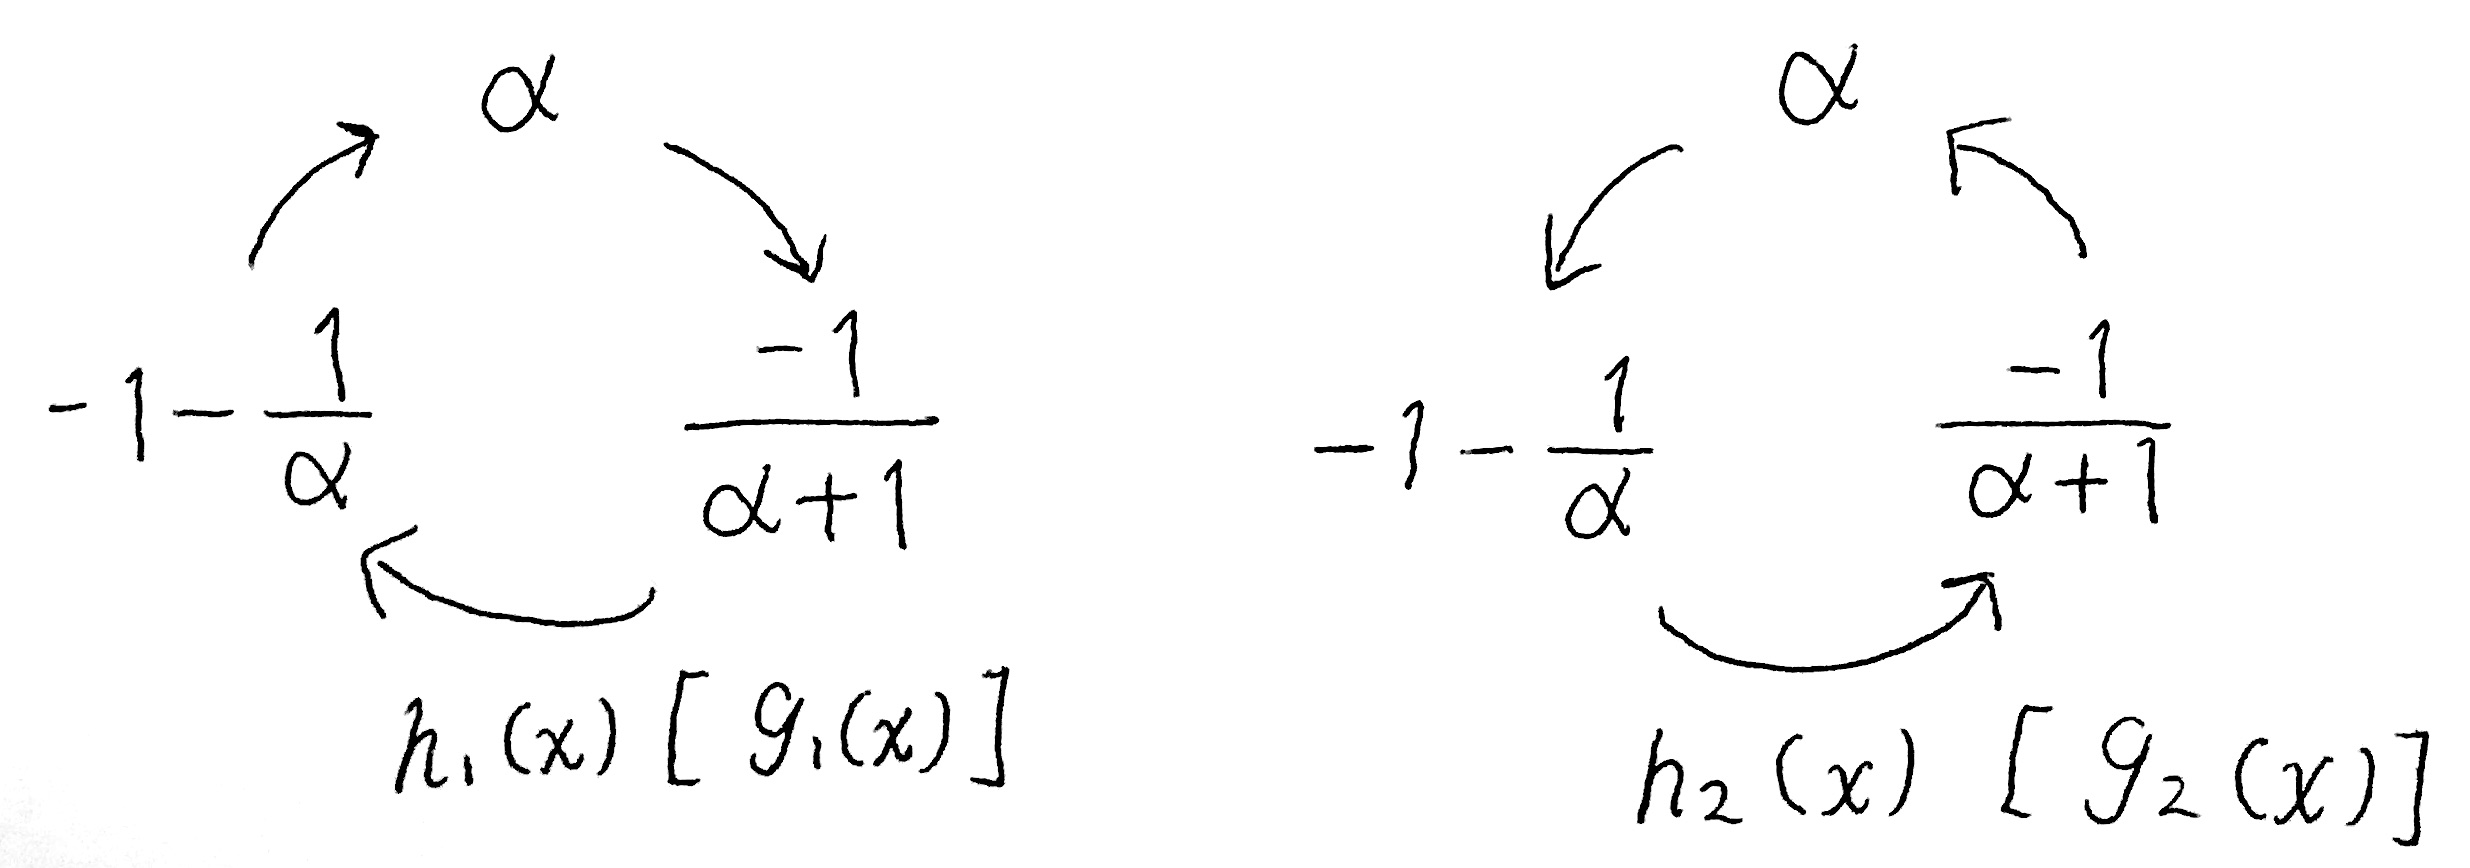
\includegraphics[width=7cm]{tuzi/image/5}
\end{figure}\noindent
と循環の方向が逆になります。\par
また、$g_1(g(g(x))) = x$ が成立するので
\begin{align*}
  \{(x^2-2)^2-2\}^2-2 = x\\
  x^8-8x^6+20x^4-16x^2-x+2 = 0
\end{align*}
よって
\[
(x^3+x^2-2x-1)(x^3-3x+1)(x+1)(x-2) = 0
\]
よって、$x^3-3x+1 = 0$は$g_1(x) = x^2-2$を循環式として持ちます。もう一つの循環式は$g_3(x)=-x^2-x+2$となり、一次分数関数の形では、それぞれ$h_3(x) = \frac{x-1}{x},h_4(x) = \frac{1}{1-x}$となります。$\alpha$を代入してみると
\begin{figure}[H]
  \centering
  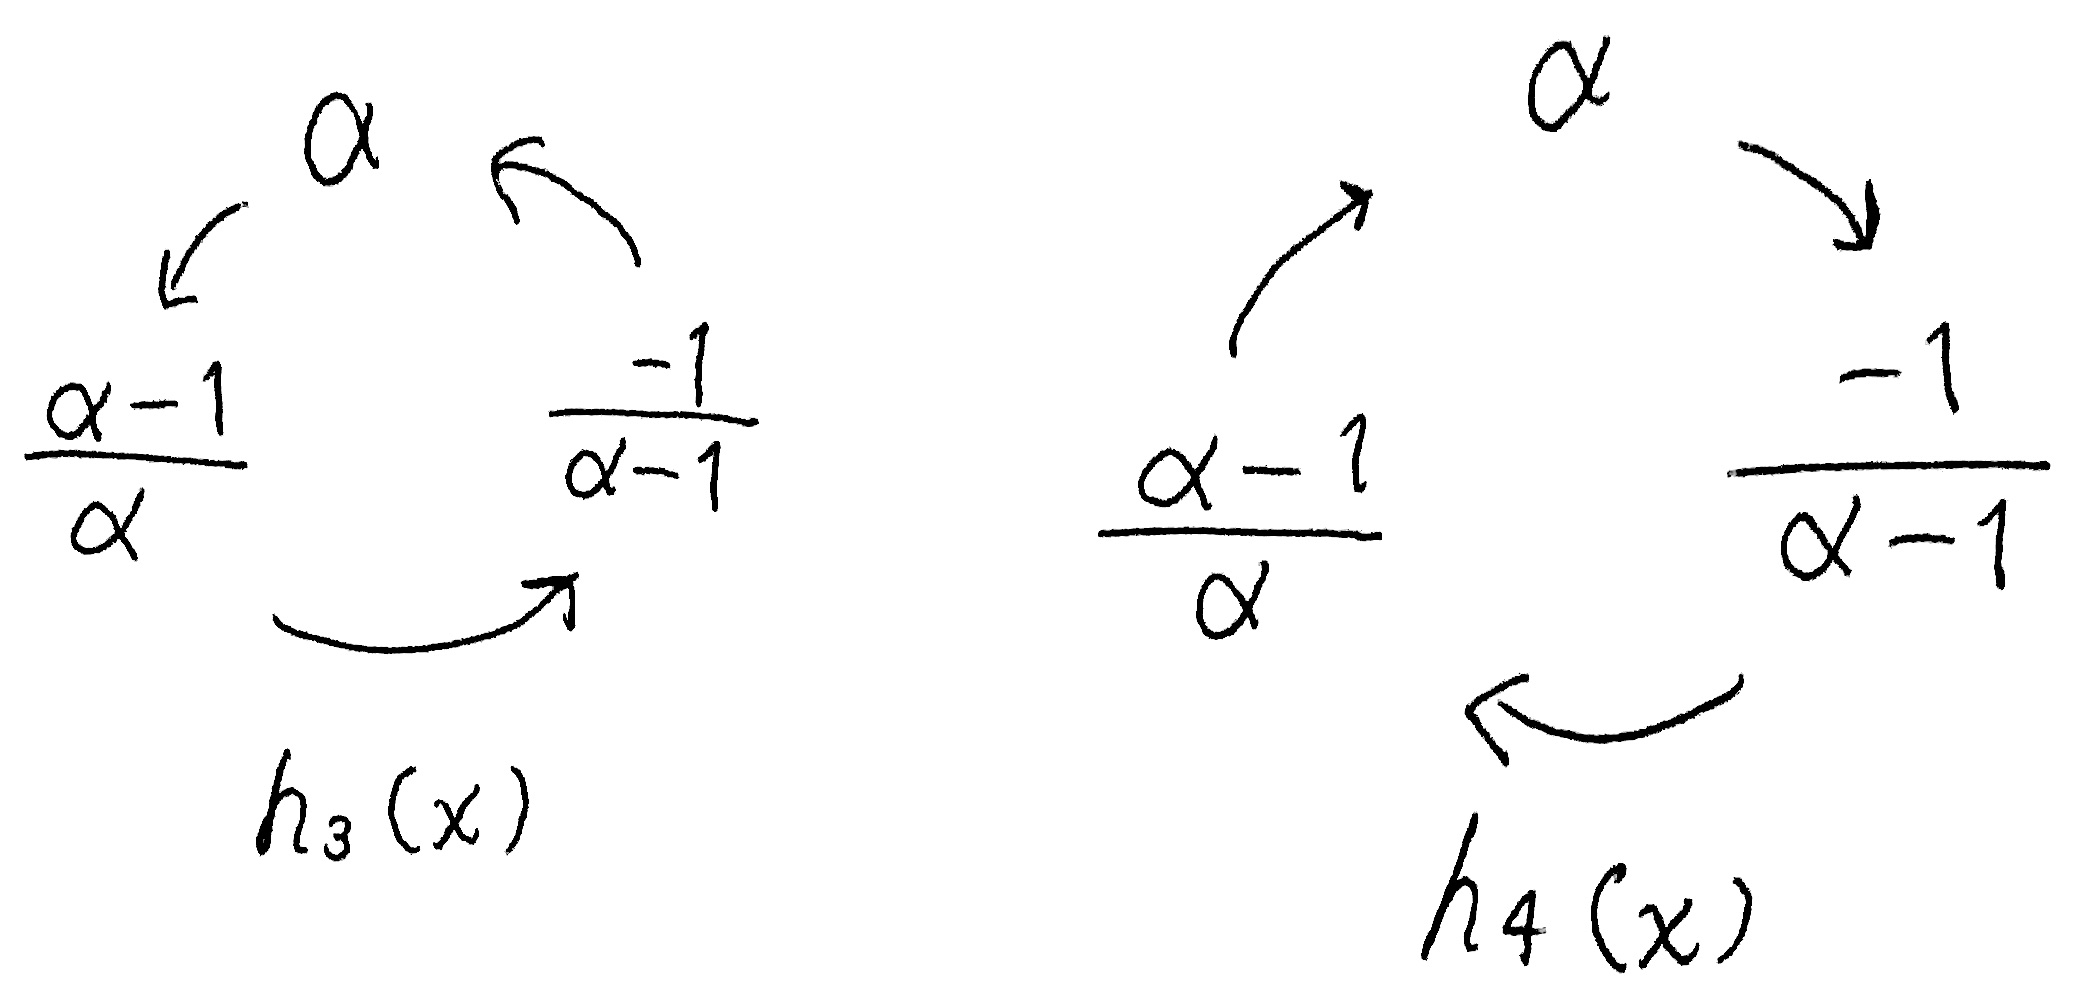
\includegraphics[width=7cm]{tuzi/image/6}
\end{figure}\noindent
となり循環しているのが確かめられました。\par
ちなみに$x+1 = 0,x-2=0$の解を$g_1(x)$に代入しても同じ解が得られます。

%
\section*{最後に一つ確認問題を}
\begin{screen}
  $x^3-6x^2+11x-6 = 0$の解と解の循環式を求め、循環することを確かめよ
\end{screen}
%
\subsection*{解答}\vspace{-3zw}
\begin{align*}
  & x= 1,2,3,\\
  & g_1(x)=-\frac{3}{2}x^2+\frac{11}{2}-2,\\
  & g_2(x) =\frac{3}{2}x^2-\frac{13}{2}x+8,\\
  & h_1(x)=\frac{10x-26}{6x-14},\\
  & h_2(x) = \frac{14x-26}{6x-10}
\end{align*}

\begin{figure}[H]
  \centering
  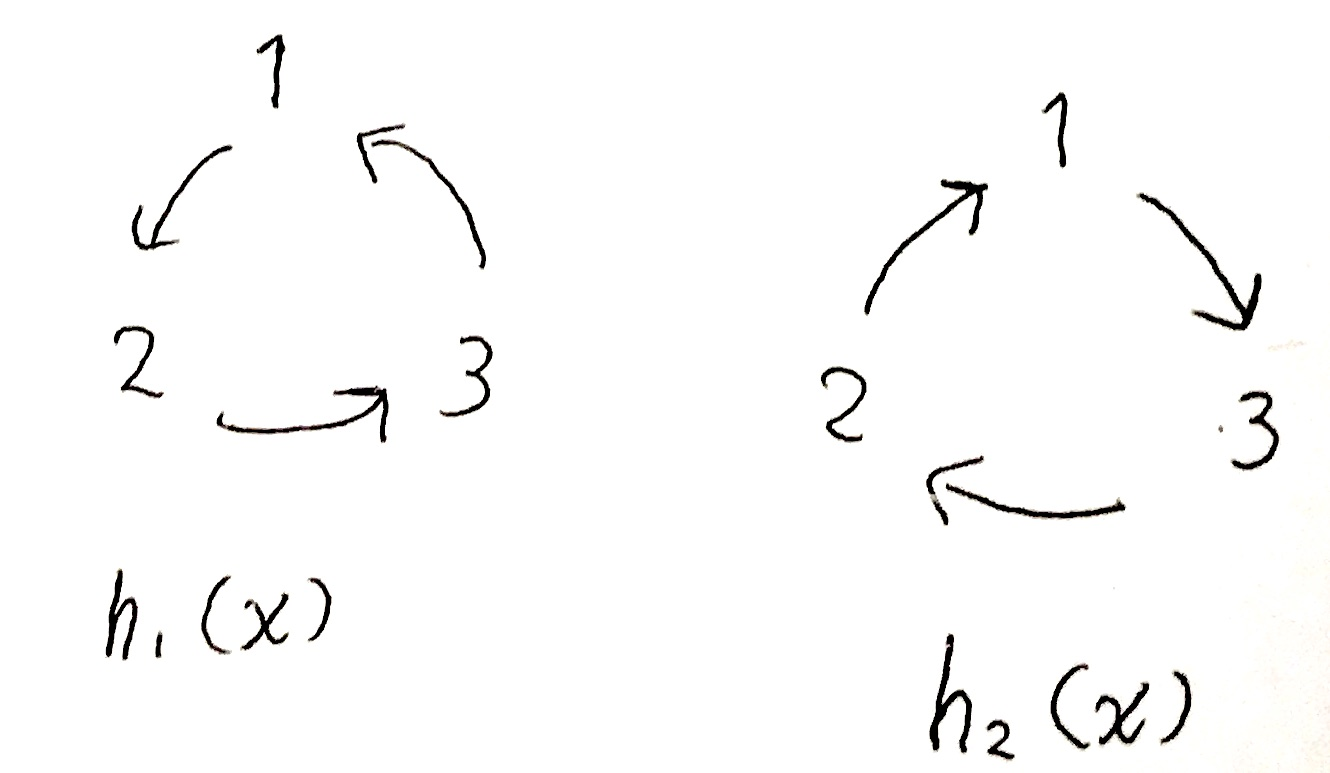
\includegraphics[width=6cm]{tuzi/image/7}
\end{figure}

%参考文献
%thebibliographyは使わないでください。\chapterになっちゃう!
\section*{参考文献}
\begin{enumerate}
  \item 解の巡回,\,「\url{http://www.004.upp.so-net.ne.jp/s_honma/solution/}\url{solution3.html}」
  \item 早稲田大学理工学部の入試問題
\end{enumerate}






%
